% Report on the competition template (template.tex of the organisers): acmart sigconf, preamble.tex, main.bib.
% Numbers marked \valPQ etc. come from figures/numbers.tex, written by report/figures.py from the pipeline outputs.
\documentclass[sigconf,nonacm]{acmart}
% Packages and settings for report.tex (the competition template loads this file after \documentclass[sigconf]{acmart}).
\usepackage{xcolor}
\usepackage{graphicx}
\usepackage{booktabs}
\usepackage{multirow}
\usepackage{enumitem}

% Gray guide text of the template: \guide{...} is shown only while \guideStyletrue is set.
\newif\ifguideStyle
\newcommand{\guide}[1]{\ifguideStyle{\color{gray!65}\itshape #1}\fi}

% No ACM publication boilerplate (report.tex also passes the nonacm class option): this is a competition report.
\settopmatter{printacmref=false}
\renewcommand\footnotetextcopyrightpermission[1]{}

\newcommand{\valPQ}{0.462}
\newcommand{\valSQ}{0.692}
\newcommand{\valRQ}{0.667}
\newcommand{\valLo}{0.441}
\newcommand{\valHi}{0.483}
\newcommand{\valTP}{1,125}
\newcommand{\valFP}{470}
\newcommand{\valFN}{652}
\newcommand{\valPQone}{0.461}
\newcommand{\valPQtwo}{0.469}
\newcommand{\valPQthree}{0.459}
\newcommand{\testInstances}{1,116}
\newcommand{\agIoU}{0.61}
\newcommand{\agDice}{0.74}
\newcommand{\agTruthOne}{77}
\newcommand{\agTruthNone}{20}
\newcommand{\agTruthMany}{2.5}
\newcommand{\agPredOne}{85}
\newcommand{\agPredNone}{12}
\newcommand{\agPredMany}{3.3}
\newcommand{\multiPQ}{0.462}
\newcommand{\multiSQ}{0.690}
\newcommand{\multiIoU}{0.60}
\newcommand{\annPQ}{0.344}
\newcommand{\annSQ}{0.638}
\newcommand{\annIoU}{0.53}
\newcommand{\annDice}{0.67}
\newcommand{\annTruthOne}{79}
\newcommand{\fpMulti}{322}
\newcommand{\multiImages}{59}
\newcommand{\fpOther}{56}
\newcommand{\consOneN}{245}
\newcommand{\consOneR}{0.31}
\newcommand{\consTwoN}{206}
\newcommand{\consTwoR}{0.72}
\newcommand{\consThreeN}{287}
\newcommand{\consThreeR}{0.89}
\newcommand{\sizeAN}{738}
\newcommand{\sizeAR}{0.54}
\newcommand{\sizeBN}{591}
\newcommand{\sizeBR}{0.69}
\newcommand{\sizeCN}{343}
\newcommand{\sizeCR}{0.73}
\newcommand{\sizeDN}{105}
\newcommand{\sizeDR}{0.65}


\guideStylefalse

\begin{document}

\title{Box-Prompted Segmentation of Solar Filaments}
\subtitle{A Solution to the Solar Filament Segmentation Challenge 2026} % DO NOT CHANGE

\author{Artem Shelamanov}
\email{artdoctorka@gmail.com}

\begin{abstract}
    This report describes our solution to the Solar Filament Segmentation Challenge~2026, a Kaggle competition on automatic segmentation of solar filaments in GONG H-$\alpha$ observations. We split the task into detection and segmentation. Four YOLO26s detectors, each trained on a different three quarters of the training images, propose a box for every filament. A U-Net with a ResNet18 encoder then segments the filament inside each box, using an image crop and a binary mask of the box as input. The candidates of the four detectors are merged, and a greedy selection keeps a fixed number of non-overlapping instances per image. On a validation fold that none of the models saw during training, the pipeline reaches a Panoptic Quality of \valPQ{} (95\% interval \valLo--\valHi); on the images of that fold with several annotations, one annotator scored against another reaches only \annPQ{}. The submitted predictions score 0.40 on the public leaderboard. The code, the trained weights and a notebook that runs every step are publicly available.
\end{abstract}

\maketitle

% ==================================== %
%              INTRODUCTION            %
% ==================================== %
\section{Introduction}
    This report goes over the details of our submitted solution to the Solar Filament Segmentation Challenge~2026 \cite{filament-segmentation-2026}. The challenge, launched on July~10,~2026, is organized by the Earth-Space AI Research (ESAIR) Lab\footnote{\href{https://www.esairlab.com/home}{www.esairlab.com/}}. This challenge utilizes the MAGFiLO dataset for evaluation of the segmentation algorithms \cite{ahmadzadeh2024dataset}.

    Two properties of the challenge determined our design. The first is the metric. Panoptic Quality (PQ) \cite{kirillov2019panoptic} scores individual filaments rather than pixels: a predicted filament counts only if its mask overlaps an annotated filament with an IoU above 0.5, and every unmatched prediction or annotation costs the same. Earlier deep-learning work on H-$\alpha$ filaments used U-Net variants for pixel-wise segmentation \cite{liu2021filament} and Mask R-CNN for instance segmentation \cite{ahmadzadeh2019toward}. The second property is that an image can carry up to three independent annotations, and the metric scores a prediction against each of them separately. The annotators often disagree. On our validation images with more than one annotation, one annotator scored against another reaches a PQ of only \annPQ{}. A good prediction therefore contains the filaments that annotators tend to agree on, outlined the way a typical annotator would outline them.

    Our pipeline has two stages (Figure~\ref{fig:pipeline}). An ensemble of detectors finds the filaments, and a box-prompted U-Net segments each of them from a crop at full resolution. A final selection step decides how many instances to predict per image, which matters for PQ because false positives and false negatives carry equal weight. The code, the trained weights and a notebook are available at \url{https://github.com/ArtDoctor/solar-kaggle-public}.

% ==================================== %
%              METHODOLOGY             %
% ==================================== %
\section{Methodology}\label{sec:methodology}

\begin{figure*}[t]
  \centering
  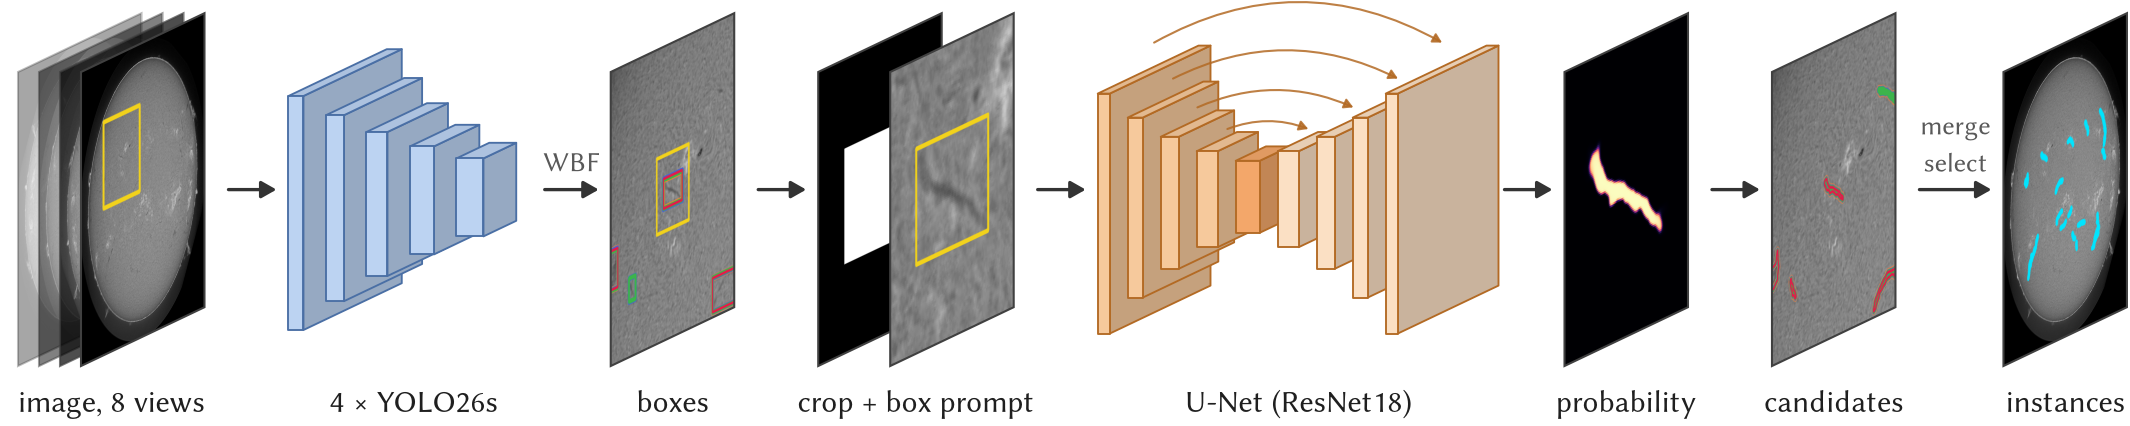
\includegraphics[width=\textwidth]{figures/pipeline.png}
  \caption{The pipeline on a test image. Four detectors propose boxes (one colour per detector). Each box becomes a crop with a box prompt, which the U-Net turns into a mask probability. The candidates of all detectors are merged and selected without overlap.}
  \label{fig:pipeline}
\end{figure*}

\subsection{Data, splits and preprocessing}
    The training set contains 707 images of $2048\times2048$ pixels with 1,154 annotator records and 8,199 filament polygons. The test set contains 180 images. We rasterised the polygons with the COCO mask tools. For validation we split the training images into four folds by calendar month (156, 182, 185 and 184 images). Images taken a few days apart show the same filaments, and a random split would place such near-duplicates on both sides. Fold~0 is our validation set throughout; the four folds are also used to train the detectors out of fold (Section~\ref{sec:detection}).

    We use the images as they are. The detector receives the grayscale image copied into three channels, and the mask model receives it normalised with the mean and standard deviation of ImageNet averaged over the colour channels (0.449 and 0.226). A limb-darkening correction did not increase filament contrast in our measurements, so we did not apply it. The models use the pixels only: no file names, dates, observatories or annotator identities, and no external data apart from ImageNet and COCO pre-training.

\subsection{Detection}\label{sec:detection}
    We fine-tune the COCO-pretrained YOLO26s detector \cite{ultralytics} four times, each time on three of the four folds. The detector is trained on tiles of $1024$ pixels cut at native resolution ($3\times3$ tiles per image with a stride of 512 pixels), so that thin filaments are not lost to downscaling. Every combination of a tile and an annotator record is a separate training sample, labelled with that annotator's filaments in the tile; a filament is labelled if at least 30 of its pixels and a quarter of its area lie inside the tile. Tiles without filaments are kept with probability 0.3. The labels are polygons rather than boxes, which keeps the boxes tight under rotation augmentation. Training runs for 12 epochs with AdamW (batch 8, learning rate $10^{-3}$ with cosine decay to $2\cdot10^{-5}$) and uses flips, rotations of up to $15^\circ$, scaling by up to 25\%, translation by up to 10\% and brightness changes.

    At inference each detector processes the full image at two input sizes, 2048 and 1280 pixels, each with the four combinations of horizontal and vertical flips. The eight box sets are fused by weighted box fusion \cite{solovyev2021wbf} at an IoU of 0.45. A fused box is the score-weighted mean of its members, and its score is the sum of the member scores divided by the number of views, so a box that appears in only one of the eight views keeps an eighth of its score.

\subsection{Box-prompted mask model}
    For every box we cut a square crop centred on the box with side $s + 2\max(32, 0.3s)$, where $s$ is the longer side of the box, and letterbox it to $512\times512$ pixels. The network input has two channels: the normalised crop and a binary mask of the box. The model is a U-Net \cite{ronneberger2015unet} with an ImageNet-pretrained ResNet18 encoder \cite{he2016resnet,iakubovskii2019smp}. It outputs, for every pixel, the probability that the pixel belongs to the filament in the box. The box channel tells the network which of several neighbouring filaments to segment, much like the box prompts of SAM \cite{kirillov2023sam}.

    The training crops are prompted with the boxes that each detector produces on its held-out fold, so that the prompts seen in training resemble those at test time. For each annotated filament we take the detector box with the highest IoU among the 40 best boxes of the image, provided that this IoU is at least 0.3 and that the whole filament fits inside the crop; otherwise we use the filament's own bounding box. The two highest-scoring boxes whose crops contain no annotated pixel of any annotator become negative examples with an empty target. In every epoch we draw one annotator record per image and use its crops together with the negative crops of that image. The model thus learns the outlines of individual annotators rather than their union. We train for 24 epochs with AdamW (batch 16, learning rate $3\cdot10^{-4}$ with cosine decay, weight decay $10^{-4}$) on the sum of binary cross-entropy and soft Dice loss. For augmentation, each edge of the prompt box is moved at random by up to 25\% of the box size, and the crops are flipped, rotated by multiples of $90^\circ$ and changed in contrast and brightness.

    At inference the mask model runs on the 40 best boxes of each detector and image. The probabilities are averaged over four flips, mapped back to the original crop and thresholded at 0.40. The largest 8-connected component becomes the candidate mask, and candidates smaller than 150 pixels are discarded.

\subsection{From candidates to instances}
    Most filaments are found by all four detectors, so each has up to four slightly different candidates. We visit the candidates in order of score and add each one to an earlier object if their masks overlap with an IoU above 0.5; each detector contributes at most one candidate to an object. The score of an object is the mean confidence of the four detectors, where a detector that missed the object contributes zero. Its mask is that of its highest-scoring candidate.

    The objects are then selected greedily in order of score. Each object loses the pixels already taken by earlier objects and keeps the largest remaining piece. It is dropped if this piece is smaller than 150 pixels or than 40\% of the original mask, or if the mask duplicates one that is already kept (IoU of at least 0.8). Kept pieces less than 8 pixels apart are merged into one instance, which joins filaments that the mask model broke into fragments. The output is pixel-disjoint, so an annotated filament can match at most one prediction. The score cutoff is found by bisection so that the test set receives 6.2 instances per image on average, the density with the highest validation PQ (Figure~\ref{fig:density}).

\subsection{Implementation and runtime}
    The pipeline is about 800 lines of Python built on PyTorch~2.8, Ultralytics~8.4 and Segmentation Models PyTorch~0.5. On one NVIDIA RTX~4070 with 12~GB of memory, each detector trains in 23 minutes and the mask model in 30 minutes. The full pipeline, from the raw data to the submission file, takes about 2.5 hours, plus half an hour for the validation mask model. Inference on the 180 test images takes about 15 minutes, or 5 seconds per image. With the released weights the code reproduces the submitted file byte for byte, which we checked on a fresh copy of the repository.

\begin{figure*}[t]
  \centering
  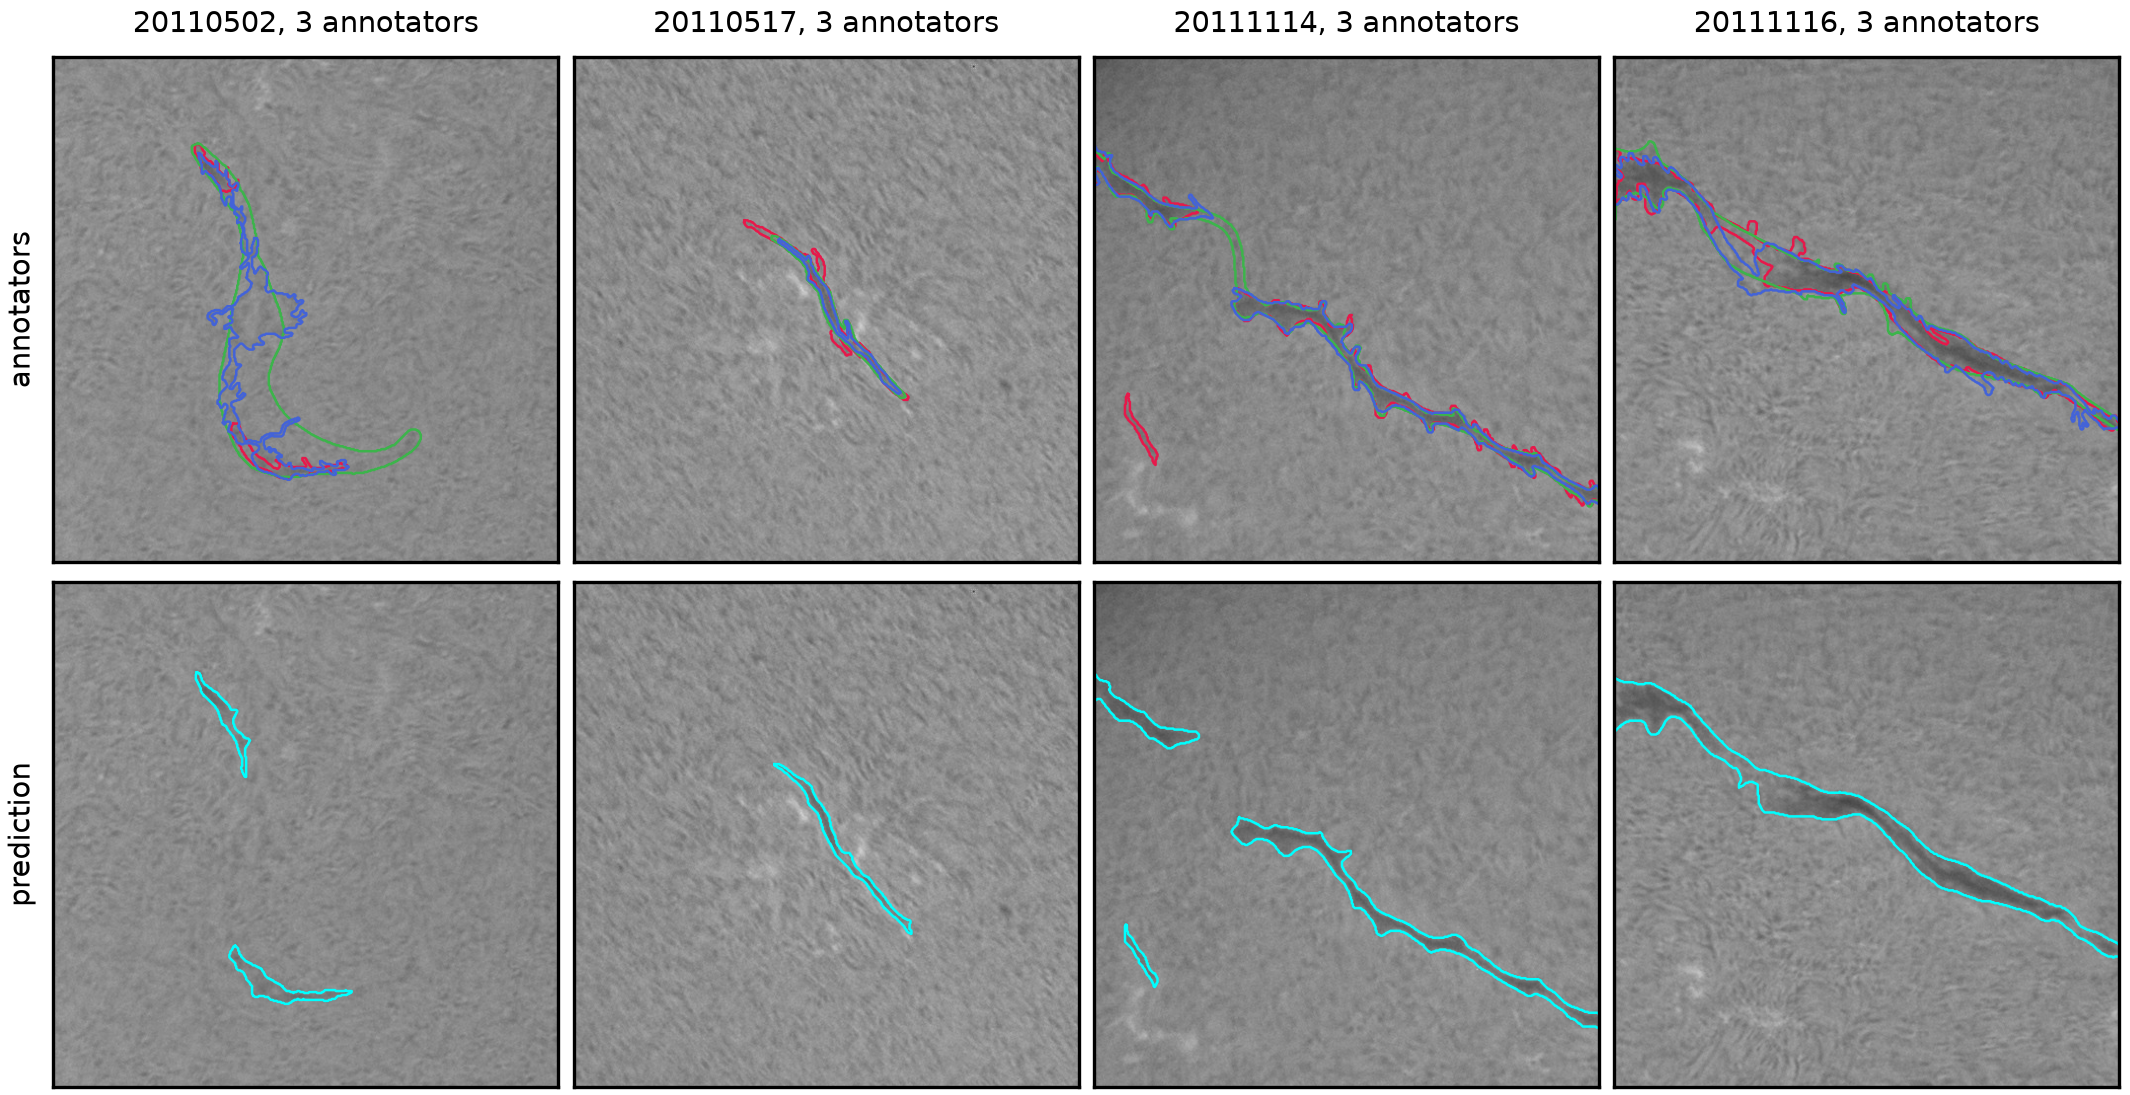
\includegraphics[width=\textwidth]{figures/examples.png}
  \caption{Validation images (fold 0, not seen in training) with three annotators each. Top: the outlines of the annotators, one colour per annotator. Bottom: our instances.}
  \label{fig:examples}
\end{figure*}

% ==================================== %
%              EVALUATION              %
% ==================================== %
\section{Evaluation}\label{sec:evaluation}

\subsection{Protocol}
    All validation numbers are computed on fold~0. Its boxes come from the detector trained on folds 1--3, and its masks from a mask model trained without fold~0, whose training crops are prompted with the boxes of detectors 1--3; no model has seen these images. The other three detectors were trained on fold~0, so validation uses one detector while the submission uses all four. PQ is computed as in the organisers' self-evaluation notebook. Within each annotator record, a pair of an annotated and a predicted mask with an IoU above 0.5 is a true positive, unmatched predictions are false positives, and unmatched annotations are false negatives. The counts and IoUs are pooled over all records. We report 95\% bootstrap intervals over images (2,000 resamples), and paired bootstrap intervals for differences between variants.

\subsection{Results}
    Table~\ref{tab:results} gives the validation score at the submission density. Images with one, two and three annotator records score about the same. The PQ curve over the number of instances per image peaks at 6.2 and stays within 0.005 of its maximum between 5.4 and 7.0 (Figure~\ref{fig:density}). Leaderboard submissions at other densities during development agreed with this curve (4.9 per image: 0.39, 6.4: 0.39, 8.3: 0.38). Training noise is of the same order as many of the effects we measure: three mask models trained with this recipe in separate runs scored 0.462 (the run reported here), 0.466 and 0.468 on the same validation boxes. The test submission has \testInstances{} instances on 180 images and scores 0.40 on the public leaderboard.

\begin{table}[t]
  \caption{Validation results (fold 0, 156 images, 248 annotator records) at 6.2 instances per image.}
  \label{tab:results}
  \begin{tabular}{lr}
    \toprule
    PQ (95\% interval) & \valPQ{} (\valLo--\valHi) \\
    SQ / RQ & \valSQ{} / \valRQ{} \\
    TP / FP / FN & \valTP{} / \valFP{} / \valFN{} \\
    PQ on images with 1 / 2 / 3 records & \valPQone{} / \valPQtwo{} / \valPQthree{} \\
    Public leaderboard (test) & 0.40 \\
    \bottomrule
  \end{tabular}
\end{table}

\begin{figure}[t]
  \centering
  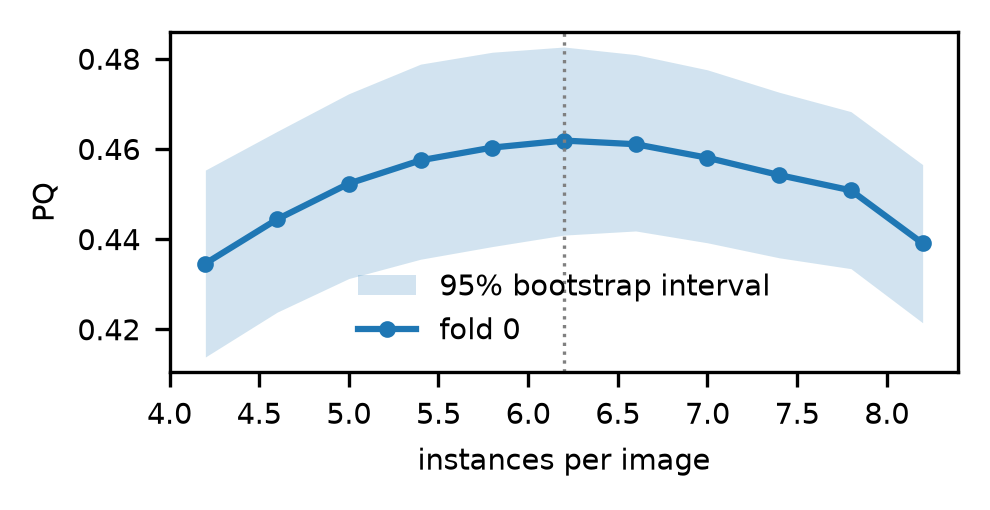
\includegraphics[width=\columnwidth]{figures/density.png}
  \caption{Validation PQ against the number of instances per image. The dotted line marks the submission density.}
  \label{fig:density}
\end{figure}

\begin{figure*}[t]
  \centering
  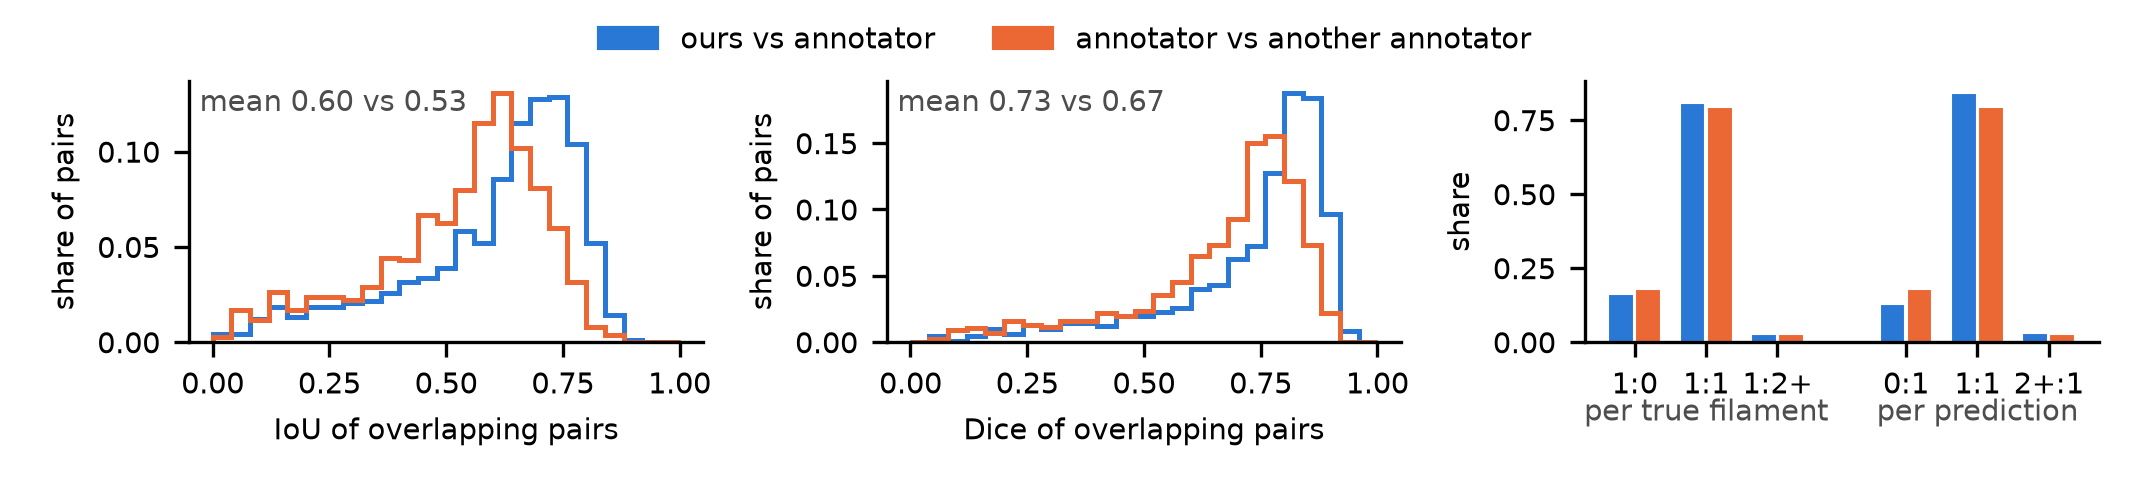
\includegraphics[width=\textwidth]{figures/agreement.png}
  \caption{The statistics of the organisers' self-evaluation notebook on the \multiImages{} validation images with two or three annotators, for our predictions against each annotator and for each annotator against another. Left and middle: IoU and Dice of all overlapping pairs. Right: annotated filaments overlapped by 0, 1 or more predictions (1:$n$) and predictions overlapping 0, 1 or more annotated filaments ($n$:1).}
  \label{fig:agreement}
\end{figure*}

\subsection{Agreement with the annotators}
    The organisers' rubric also considers the distributions of IoU and Dice and the one-to-many and many-to-one relations between annotated and predicted filaments. Over all validation images, the pairs of a prediction and an annotated filament that overlap have a mean IoU of \agIoU{} and a mean Dice of \agDice{}. Of the annotated filaments, \agTruthOne\% overlap exactly one prediction, \agTruthNone\% overlap none and \agTruthMany\% overlap two or more; \agPredOne\% of the predictions overlap exactly one annotated filament and \agPredMany\% overlap two or more.

    Figure~\ref{fig:agreement} compares these statistics with the agreement between annotators. Our predictions agree with each annotator more closely than the annotators agree with each other: on the images with several annotators, PQ is \multiPQ{} for our predictions and \annPQ{} between annotators, and the mean IoU of overlapping pairs is \multiIoU{} against \annIoU{}. The relations are almost the same in both cases. The model has, in effect, learned an average outline, which lies closer to each annotator than one annotator's outline lies to another's.

\subsection{Error analysis}
    Table~\ref{tab:errors} breaks recall, the share of annotated filaments matched with an IoU above 0.5, down by annotator agreement and by size. On images with three annotators we find \consThreeR{} of the filaments drawn by all three, \consTwoR{} of those drawn by two and \consOneR{} of those drawn by only one. Many of our false positives are of the same kind: on images with several annotators, \fpOther\% of the predictions that match nothing in one record match a filament in another. Recall is lowest for filaments below 1,000 pixels and falls again for the largest ones. Long filaments are often covered only in part or split into pieces too far apart for the 8-pixel merge (Figure~\ref{fig:examples}, first column).

\begin{table}[t]
  \caption{Validation recall (IoU above 0.5) by the number of annotators who drew a filament (images with three records) and by filament area.}
  \label{tab:errors}
  \small
  \begin{tabular}{@{}lrr@{}}
    \toprule
    Annotated filaments & Count & Recall \\
    \midrule
    Drawn by 3 of 3 annotators & \consThreeN & \consThreeR \\
    Drawn by 2 of 3 annotators & \consTwoN & \consTwoR \\
    Drawn by 1 of 3 annotators & \consOneN & \consOneR \\
    \midrule
    Area below 1,000 px & \sizeAN & \sizeAR \\
    Area 1,000--2,500 px & \sizeBN & \sizeBR \\
    Area 2,500--6,000 px & \sizeCN & \sizeCR \\
    Area above 6,000 px & \sizeDN & \sizeDR \\
    \bottomrule
  \end{tabular}
\end{table}

\subsection{Ablations and alternatives}
    Table~\ref{tab:ablation} lists what each part of the pipeline contributes. The components are worth between 0.002 and 0.02 PQ each, several of them less than the training noise, and none decides the result on its own. A larger variant with a second detector family and a gradient-boosted re-scorer of the candidates was 0.0075 better on validation (interval 0.000 to 0.015) but scored the same 0.40 on the public leaderboard, so we removed it to keep the pipeline simple.

    Before settling on this design we tried several others. Scored early in the project against the first annotator record of each fold-0 image only (so not comparable with Table~\ref{tab:results}), classical thresholding of dark structures reached a PQ of 0.110 with about nine false positives per true positive, SAM~2.1 \cite{ravi2025sam2} prompted with our boxes but not fine-tuned 0.249, a full-disk U-Net with connected components 0.336, and Mask R-CNN \cite{he2017maskrcnn} 0.338, against 0.414 for the first version of our two-stage pipeline.

\begin{table}[t]
  \caption{Development ablations on fold 0: PQ change of each modification against one detector with every other part in place, at 6.2 instances per image (95\% paired bootstrap interval over images).}
  \label{tab:ablation}
  \small
  \begin{tabular}{@{}lr@{}}
    \toprule
    Change & $\Delta$PQ \\
    \midrule
    Detection in one view (2048 px, no flips) & $-0.006$ ($-0.016$, $+0.004$) \\
    Detection in one view (1280 px, no flips) & $-0.020$ ($-0.029$, $-0.010$) \\
    Detection in two views (both sizes, no flips) & $-0.002$ ($-0.009$, $+0.005$) \\
    No flip averaging of mask probabilities & $-0.005$ ($-0.010$, $-0.001$) \\
    No merging of fragments ($\le8$ px) & $-0.007$ ($-0.013$, $-0.001$) \\
    Adding a second detector family & $+0.005$ ($-0.001$, $+0.011$) \\
    Detectors trained 30 instead of 12 epochs & $-0.000$ ($-0.009$, $+0.008$) \\
    Mask model trained 12 instead of 24 epochs & $-0.004$ ($-0.009$, $+0.001$) \\
    \bottomrule
  \end{tabular}
\end{table}

\subsection{Strengths, weaknesses and improvements}
    The pipeline is small: two model types with one training recipe each, about 2.5 hours of training on a single consumer GPU, and five seconds of inference per image. Its predictions never overlap each other, \agTruthOne\% of the annotated filaments are covered by exactly one prediction, and its outlines agree with each annotator more closely than the annotators agree with each other.

    The main weakness is the filaments that only one annotator drew, of which we find fewer than a third. This is partly unavoidable, since the other annotators of the same image did not consider these structures filaments either. Long filaments are a second weakness. The mask model sees one crop per box and often stops short of faint ends or breaks the filament into pieces. A model with a wider field of view, or one that first traces the filament spine and then predicts its width, could address this. Finally, the public leaderboard score is about 0.06 below validation. MAGFiLO was annotated by 24 groups \cite{ahmadzadeh2024dataset}, only 19 of which appear in the training data, and on our folds the PQ of individual groups ranges from 0.42 to 0.53. Since a classifier could not tell test images from training images, we attribute the gap to the annotation style of the unseen groups. Choosing the number of instances per image adaptively and training on consensus targets instead of individual records are the improvements we would try next.

% ==================================== %
%            ACKNOWLEDGMENT            %
% ==================================== %
\section{Acknowledgment}\label{sec:acknowledgment}
    % Do not change
    The organization of the Filament Segmentation Challenge 2026 is partially supported by the U.S. National Science Foundation (NSF) under Grant No. 2209912 and 2433781, directorate for Computer and Information Science and Engineering (CSE), and Office of Advanced Cyberinfrastructure (OAC), and Grant No. 2511630, AST Division Of Astronomical Sciences and MPS Directorate for Mathematical and Physical Sciences.

    The Filament Segmentation Challenge 2026 is sponsored by the U.S. National Science Foundation (NSF) National Solar Observatory (NSO).

    This work utilizes GONG data obtained by the NSO Integrated Synoptic Program, managed by the National Solar Observatory, which is operated by the Association of Universities for Research in Astronomy (AURA), Inc. under a cooperative agreement with the National Science Foundation and with contribution from the National Oceanic and Atmospheric Administration. The GONG network of instruments is hosted by the Big Bear Solar Observatory, High Altitude Observatory, Learmonth Solar Observatory, Udaipur Solar Observatory, Instituto de Astrofísica de Canarias, and Cerro Tololo Interamerican Observatory.

\bibliographystyle{ACM-Reference-Format}
\bibliography{main}

\end{document}
